\chapter{Analysis of selected models}
\label{cha:analysis_of_selected_models}

\section{Spatial reproduction number model}%
\label{sec:spatial_reproduction_number_model}

\begin{enumerate}
    \item essentially the Regional model presented in ECMI
\end{enumerate}

\section{Regional growth factor model}%
\label{sec:regional_growth_factor_model}

\section{Nowcasting hospitalizations}%
\label{sec:nowcasting_hospitalizations}
\subsection{Context}
Judging the severity of the COVID-19 epidemic has been an ongoing challenge since its inception. As immunization against COVID-19 rose, strict enforcement of social distancing rules eased and testing regimes became less strict, case incidences became a less reliable and harder to interpret indicator of epidemic severity. Instead more direct indicators of morbidity, such as the number of deaths and ICU admissions and occupancy have come to the fore. But these indicators are late due to the substantial delays between infection and occurence. An alternative indicator that captures the morbidity caused by COVID-19 but is earlier than the others is the number of hospitalisations of positive COVID-19
cases.

While hospitalisations occur earlier, they still come with substantial delay between the infection and subsequent admission to hospital. Additional difficulties arise due to delays in reporting, i.e.~the time it takes until the hospital reports the new case to the national health authorities. The problem of accounting for delays in reporting for occurred, but not yet reported events has been termed \textbf{nowcasting}, i.e.~forecasting of the indicator at time ``now''. Predicting the number of hospitalisations is thus a mixture of both forecasting --- which reported COVID-19 cases will end up in the hospital --- and nowcasting --- which cases have yet to be reported --- and we will use the term nowcasting in this paper to mean this predictive mixture. In this section we focus on the situation in Germany where data on hospitalisations has been available since April 2021 provided by the German federal health care authorithy, the \gls{rki}, via Github \cite{RobertKoch-Institut2021COVID19Hospitalisierungen}. In these data the number of hospitalisations is linked to the date of reporting of the associated case, so the term of nowcasting is accurate: we are interested in the ``true'' value of the indicator today, that will only be observed after a long delay. While this association requires a careful interpretation of the indicator (see \Cref{subsec:nowcasting_discussion}) it was, besides case incidences and ICU occupancy, one of the main official indicators in Germany informing countermeasures in 2021 and so there is merit in nowcasting it. 

The extent of delays is visible in \cref{fig:delays_in_reporting}: the reported number of hospitalisations will roughly double over the course of twelve weeks. By the aforementioned reporting scheme of hospitalisations there are two reporting dates for a single hospitalised case: the reporting date of the case, i.e.~the date when local health authorities were made aware of the positive test, and the reporting date of the hospitalisation, i.e.~when the hospitalisation was reported to the \gls{rki}. This induces a double weekday effect in the reporting delays which we make visible in \cref{fig:double_weekday_effect}.

Compared to other approaches in the COVID-19 NowcastHub, that tended to exclusively focus on modelling the delay distribution with parametric and non-parametric models, our model sidesteps this complex delay structure by decomposing delayed hospitalisations into weekly chunks (\cref{fig:reporting_triangle}) and incorporating case data. As cases and hospitalisations are explicitly linked by the case reporting date we forecast the number of hospitalisations in each chunk based on the current incidences and past fractions of hospitalisations in a comparable weekly chunk. We additionally quantify uncertainty by prediction intervals that are informed by the past performance of our model. This makes our model straightforward to understand, easy to implement and fast to run.\todo{reformulate}

\begin{figure}

{\centering 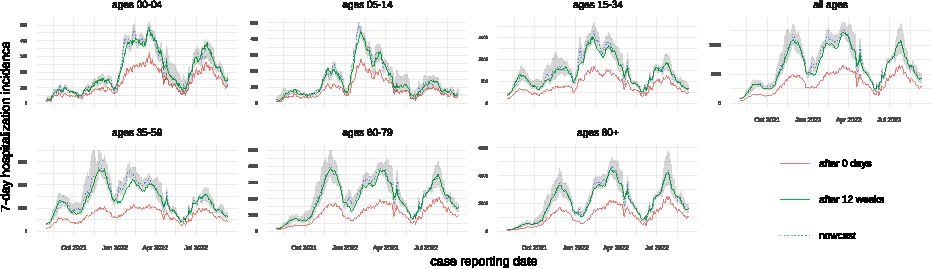
\includegraphics[width=\textwidth]{figures_tentative/delays_in_reporting-1.pdf} 

}

\caption{Germany's $7$-day hospitalisation incidence changes due to various delays such as time to hospitalisation and delays in reporting. This figure shows the extent of these delays: incidences reported at the present date (red lines) severely underestimate the hospitalisation incidence (green solid lines) that is reported after $3$ months. Our nowcasting model (blue dotted lines, 95\% prediction intervals in shaded gray) deals with this problem by predicting the hospitalisation incidence based on past cases and their delays to hospitalisation.}\label{fig:delays_in_reporting}
\end{figure}

\begin{figure}

    {\centering 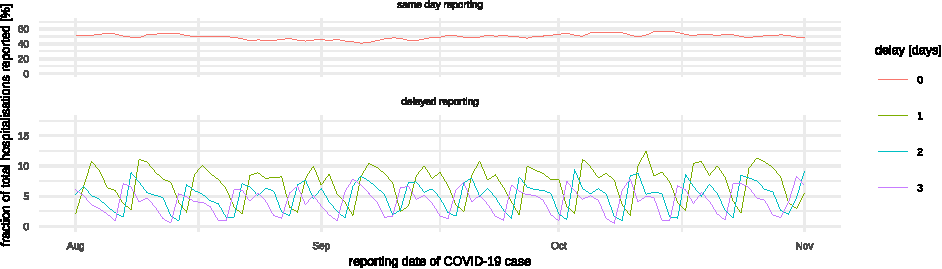
\includegraphics[width=\textwidth]{figures_tentative/double_weekday_effect-1.pdf} 

}

\caption{The hospitalisation incidence contains a double weekday effect owed to the reporting of both the COVID-19 case and the subsequent hospitalisation. While the weekday effect of the case reporting date is somewhat mitigated by summing over $7$ day periods, the weekday effect of reporting date of the hospitalisation is still present in the data. It is most pronounced for hospitalisations that are reported with delays, i.e. where the case reporting date does not match the reporting date of the hospitalisation.}\label{fig:double_weekday_effect}
\end{figure}

The origin of nowcasting lie in accounting for incurred, but not reported claims in the actuarial sciences \cite{Kaminsky1987Prediction}, delays in reporting for AIDS \cite{Zeger1989Statistical,Lawless1994Adjustments} and other infectious diseases \cite{Farrington1996Statistical}. Popular statistical approaches include methods from survival analysis \cite{Lawless1994Adjustments} and generalized linear regression \cite{Zeger1989Statistical}. In the survial analysis setting one commonly models the reverse time discrete hazard parametrically and assumes multinomial sampling of the final number of cases, potentially accounting for overdispersion. This has been studied with frequentist \cite{Midthune2005Modeling} and Bayesian \cite{Hohle2014Bayesian,AnDerHeiden2020Schatzung} methods. The generalized linear regression approach has origins in the chain ladder model from actuarial sciences \cite{Renshaw1998Stochastic} and models the observed counts in the reporting triangle by a Poisson or negative binomial distribution.
For both approaches, available covariates can be incorporated in a straightforward way. In the setting of real-time nowcasting, it is often beneficial to incorporate epidemic dynamics into the model, this can be achieved by splines \cite{Hohle2014Bayesian,vandeKassteele2019Nowcasting} or by a latent process of infections \cite{McGough2020Nowcasting}.

Nowcasting methods have wide application in accouting for reporting delays \cite{Midthune2005Modeling}, early outbreak detection \cite{Salmon2015Bayesian,Bastos2019Modelling}, and, in the recent COVID-19 epidemic, improving real-time monitoring of epidemic outbreaks \cite{AnDerHeiden2020Schatzung,Gunther2021Nowcasting,Schneble2021Nowcasting,Akhmetzhanov2021Estimation}. Evaluating a forecasting model in a real-time public health setting is advantageous as it avoid hindsight bias \cite{Desai2019Realtime}, however nowcasting approach may have difficulties with bias and properly calibrated uncertainty if used in a real-time setting. This includes rapidly changing dynamics \cite{Gunther2021Nowcasting,vandeKassteele2019Nowcasting}, both of the delay distribution and the underlying epidemic, retrospective changes in data \cite{Midthune2005Modeling} and long delays with few observed cases \cite{Noufaily2015Modelling}. 

To avoid the aforementioned hindsight bias one can make their predictions publicly available in real-time \cite{Ray2020Ensemble,Bracher2021Preregistered}. For the hospitalisations in Germany, Thomas Hotz and I have participated in the German COVID-19 NowcastHub \cite{2022Nowcasts} since November 2021 where nowcasts are available in a public Github repository \cite{2022Hospitalization} with the ``ILM-prop'' model. The ideas, especially the model and the ``double-weekday effect'', discussed this section are based on this model. However, the ``ILM-prop'' model is based on simple point estimates for the proportion of hospitalisations per reported case, neglecting regularization over time. In this thesis we extend this model to the \gls{ssm} setting of this thesis and investigate if the increased model complexity results in improved performance.

\subsection{Data}
To predict the number of hospitalisations we consider the reporting
process of both reported COVID-19 cases and reported hospitalisations.
Recall that the reporting date of a COVID-19 case is shared for both the
case and its hospitalisation, i.e.~the case and hospitalisation are
linked through this date.

As hospitalisations are only available as \(7\)-day rolling sums, we use \(7\)-day rolling sums for daily
reported incidences as well. To avoid dealing with the double weekday
effect of both reporting date of the case and reporting date of the
hospitalisation (see \cref{fig:double_weekday_effect}) we divide the
future hospitalisations we wish to predict into chunks of one week,
which gets rid of the weekday effect for the hospitalisations. This is
depicted in \cref{fig:reporting_triangle}. Our prediction of each of
these weekly chunks then consists of the fraction of hospitalisations of
reported cases in the past.

We use publicly available data from the German national health authority
(\gls{rki}) on daily reported COVID-19 cases
\cite{RobertKoch-Institut2022SARSCoV2} and weekly reported
hospitalisations
\cite{RobertKoch-Institut2021COVID19Hospitalisierungen}. Both
datasets are updated on a daily basis.

COVID-19 cases are described by their date of reporting, i.e.~the date
that the local health authorities were made aware of the case. For a
fraction (63 \%) of cases the date of symptom onset is also reported.
Due to delays in the process from infection to reporting -- e.g.~the
time it takes to get tested, evaluate the test and report the result to
local health authorities -- the date of reporting is, for most cases,
some days after symptom onset (median delay: 3 with interquartile range
\([2, 6]\)). As the date of symptom onset is not known for a substantial
amount of incident cases, and is not reported for hospitalised cases, we
focus our analysis on the date of reporting.

Hospitalisations are associated with the \emph{reporting date of the
corresponding case} and no information is available on the actual date
of hospitalisation. In addition, hospitalisations are only published as
weekly sums over the past seven days. This means that the number of
hospitalisations reported for today consists of all hospitalisations
that correspond to cases that have a \emph{case reporting date} in the
past seven days. In particular if the case reporting date of a
hospitalised case is today the case will \emph{not} count towards todays
hospitalisation count. The reporting date of hospitalisation is not
available in the dataset, but can be inferred by comparing datasets from
consecutive days.

Daily incident cases and weekly hospitalisations are reported by federal
state and age group (00-04, 05-14, 15-34, 35-59, 60-79, 80+). Incident
cases are additionally reported by county and sex.

In line with the structure of the data provided by the \gls{rki} we let \(H^a_{t,d}\) be the number of weekly hospitalisations
in age group \(a\) with case reporting date \(t - 1, \dots, t - 7\) that
are known on day \(t + d\), aggregating over all states. Accordingly we
define \(I^a_{t,d}\) to be the number of weekly incident cases in age
group \(a\) with reporting date \(t - 1, \dots, t - 7\) that are known
on day \(t + d\). Finally we reconstruct the reporting triangles for
weekly hospitalisations (\cref{fig:reporting_triangle}) by
differencing the \(H^a_{t,d}\) for fixed \(t\):
\(h^a_{t,d} = H^a_{t,d} - H^a_{t, d - 1}\), setting \(H^a_{t, -1}\) to
\(0\) by convention. We recover the reporting triangle \(i^a_{t,d}\) for
incident cases in the same manner.

\begin{figure}

    {\centering 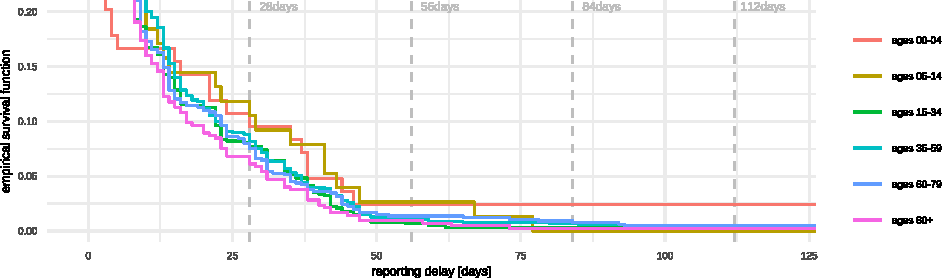
\includegraphics[width=\textwidth]{figures_tentative/delay_tails-1.pdf} 

}

\caption{Survival function of reporting delays of weekly hospitalisations $H_{t,d}$ with case reporting date 01 September 2021. The delay distribution has long tails with a non-neglibgible fraction of observed delays longer than eight weeks, in some age groups even twelve weeks.}\label{fig:delay_tails}
\end{figure}

We show the empirical surivival function of hospitalisations for a fixed
date in \cref{fig:delay_tails}. We observe that delays have long
tails, with most cases reported after 12 weeks (84 days), except for the
youngest age group. After such a long delay between infection and
hospitalisation we deem it unlikely that hospitalisation is due to COVID
and disregard all longer delays accordingly. Given such long delays, it
does not suffice to nowcast only todays hospitalisations, but also for
dates in the past to monitor hospitalisation, i.e.~observe current
trends; we thus nowcast for all delays \(d = 0, \dots, 28\).

\subsection{Model}
More formally, denote by \(h_{t,d}\) the number hospitalisations with
reporting date \(t\) that are known \(d\) days later. Unfortunately we
only observe \[H_{t,d} = \sum_{s = t - 6}^{t} h_{s,d + (t - s)},\]
i.e.~a weekly sum of reported hospitalisations. On day \(T\) our goal is
to predict \(H_{t,D}\) for large delays \(D\) and days \(t \leq T\), of
course it suffices to predict \(H_{t, D} - H_{t, T - t}\) and add the
known \(H_{t, T - t}\) to this prediction. We rewrite this into weekly
telescoping sum \[
H_{t,D} - H_{t,d} = \left(H_{t, d + 7} - H_{t,d}\right) + \left(H_{t, d + 14} - H_{t, d + 7}\right) + \dots + \left(H_{t,D} - H_{t, d + 7 K}\right),
\] where \(K = \lfloor (D -d) / 7 \rfloor\), reducing the task at hand
to predict hospitalisations in the \(k\)-th week ahead,
\(H_{t, d + 7k} - H_{t, d + 7\cdot(k - 1)}\), \(k = 1, \dots, K\). To
leverage known reported incidences, rewrite this as
\[\underbrace{\frac{H_{t, d + 7k} - H_{t, d + 7\cdot(k - 1)}}{I_{t,d}}}_{=:p_{t,d,k}} I_{t, d}\]
where \(I_{t,d}\) is the \(7\)-day case incidence with reporting date
\(t\) known at time \(t + d\), i.e.~the incidenct case analouge of
\(H_{t,d}\).

Assuming that the proportions \(p_{t,d,k}\) change slowly over time
\(t\) we estimate them by

\begin{align}
\label{eq:predict_p_tdk}
\widehat {p_{t,d,k}} = \frac{H_{t - 7k, d + 7k} - H_{t - 7k, d + 7\cdot(k - 1)}}{I_{t - 7k,d}} = p_{t - 7k,d,k}
\end{align}

and finally predict

\begin{align}
\label{eq:predict_H_tD}
\widehat{H_{t,D}} = H_{t,d} + I_{t,d} \left(\widehat{p_{t,d,1}} + \dots + \widehat{p_{t,d,K}}\right).
\end{align}

As hospitalisation is affected by age, we perform this procedure for all
available age groups separately and finally aggregate over all age
groups to obtain a nowcast for all age groups combined.

This describes our point nowcast for \(7\)-day hospitalisations. To
obtain uncertainty intervals we fit a normal (age groups 00-04 and
05-14) or lognormal (all other age groups) distribution to the past
performance of our model. We chose these distributions based on
explorative analysis and believe that these should be seen as heuristics
rather than as a matter of fact, which is in line with the philosophy of
our model to be as simple as possible.

Denote by \(\hat H_{t,D,s}\) the nowcast made for date \(t\) on date
\(s \geq t\). Starting with date \(t + D\) the definite \(H_{t,D}\) is
known and we can estimate the absolute prediction error
\(\varepsilon_{t,s} = H_{t,D} - \hat H_{t,D,s}\) and the relative
prediction error
\(\eta_{t,s} = \log \left( H_{t,D} - H_{t, s - t}\right) - \log \left( \hat H_{t,D,s} - H_{t, s- t} \right)\).
For the nowcast for date \(t\) made on date \(s\) we estimate the
standard deviation \(\hat\sigma\) of
\(\varepsilon_{t - D - i, s - D - i}\) or
\(\eta_{t - D - i, s - D - i}\) (age groups 00-04, 05-14 and others
respectively), \(i = 0, \dots, 27\) by its empirical counterpart. The
estimated predictive distribution which informs our prediction intervals
is then \(\mathcal N (\hat H_{t,D,s}, \sigma^2)\) (age groups 00-04 and
05-14) or
\(\mathcal{LN} \left( \log \left(\hat H_{t,D,s} - H_{t, s - t}\right), \sigma^2 \right) + H_{t, s - t}\)
(all other agr groups).

\begin{figure}
    \centering
    \includegraphics[width=\textwidth]{tikz/reporting_triangle}
    \caption{Decomposition of the daily reported hospitalisation incidences into the {\color{TUIl-orange} known incidences}, i.e. the \textbf{reporting triangle}, and {\color{TUIl-green}the future weekly increments}. {\color{TUIl-blue}The last increment} might not be a weekly one, but we expect few cases to occur for such long delays.}
    \label{fig:reporting_triangle}
\end{figure}

\subsection{Discussion}\label{subsec:nowcasting_discussion}
Before evaluating the predictive performance of our model we investigate
how the fraction of hospitalisations after one up to four weeks changes
over time across different age groups. 
\cref{fig:hospitalisation_probabilities_over_time} shows that these
fractions are changing slowely over time, especially in the older age
groups. Due to smaller numbers of infections and hospitalisations
reported in the younger age groups these fractions vary more strongly,
occassionally dropping to \(0\). Across all age groups we observe a
steady decline from October 2021 to December 2021 with a steeper drop in
fraction of hospitalisations starting with January 2022. The former
period corresponds to a time of mandatory testing at the workplace which
may improve ascertainment of asymptomatic and less severe cases. The
latter effect is most recognizable in the 35-59 age group and coincides
with the time that the Omicron variant became dominant in Germany
\cite{RobertKoch-Institut2022Lagebericht2022-01-20}. Additionally
there is no visually discernible weekday effect present in 
\cref{fig:hospitalisation_probabilities_over_time}.

\begin{figure}

    {\centering 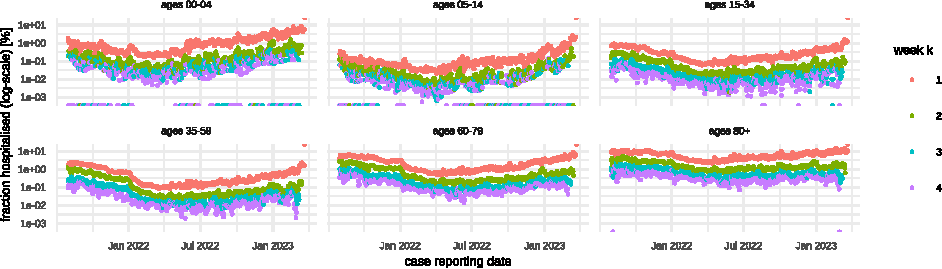
\includegraphics[width=\textwidth]{figures_tentative/hospitalisation_probabilities_over_time-1.pdf} 

}

\caption{We show the fractions of hospitalisations in the $k$-th week after case reporting date $t$  of initially reported cases in different age groups, i.e. $p_{t,0,k} = \left(H_{t,7 k} - H_{t, 7 \cdot (k - 1)}\right) / I_{t,0} $. Note the log-scale of the $y$-axis. During periods of low incidence, e.g. July -- September, we find large fluctations, but no discernable weekly pattern. With rising case numbers the fractions stabilise and decrease in most age groups. This might be due to changes in testing regime detecting less severe cases. As changes occur on slow time scales, estimating these fractions by Eq.~\eqref{eq:predict_p_tdk} is a promising approach.}\label{fig:hospitalisation_probabilities_over_time}
\end{figure}

In \cref{fig:delays_in_reporting} we depict the nowcasts produced
from our model including \(95\%\) prediction intervals, whose lengths
are based on the past performance of our model. Except for the period
from January to April 2022, the model produces reasonable nowcasts with
prediction intervals that have sensible widths. In the aforementioned
period the nowcasts overpredict the final hospitalisations, except for
the oldest age group, and, after a transitionary period, have larger
uncertainty.

\begin{figure}

    {\centering 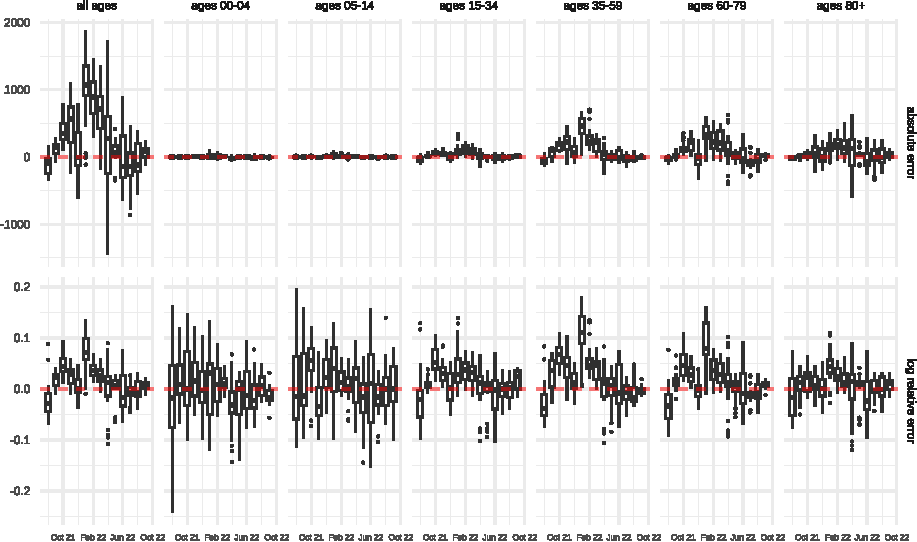
\includegraphics[width=\textwidth]{figures_tentative/REP-1.pdf} 

}

\caption{
We show relative and absolute errors of prediction of our model for same day nowcasts by month of forecast and selected age groups. 
Relative errors are displayed on the log10 scale, i.e. as $\log_{10} (\text{predicted}) - \log_{10} (\text{actual})$.
Up to December 2021 the model performs well, especially in the older age groups where most hospitalisations occur. 
The sharp increase in cases in January 2022 coupled with a lower probability of hospitalisation, most likely due to the appearance of the Omicron variant in Germany, lead to overpredictions across all age groups.
}\label{fig:REP}
\end{figure}

To investigate the quality of point predictions we display the
time-evolution of absolute (AEP) and relative errors of predictions
(REP, \(\log_{10}\)-scale) across all age groups in 
\cref{fig:REP}. From this figure one can infer that the point nowcasts
produced by our model tend to slightly overpredict the final number of
hospitalisations. Indeed, the interquartile range of REPs for all age
groups and dates combined spans \([-1.56, 8.33]\), demonstrating the
same tendency. The highest REPs occured in October / November 2021 and
January/February 2022; the first corresponding to introduction of
mandatory testing at the workplace and the second to the arrival of the
Omicron variant in Germany. In both circumstances the number of cases
rose while hospitalisations did not increase proportionally, a similar
effect to the one observed in 
\cref{fig:hospitalisation_probabilities_over_time}.

\begin{figure}

    {\centering 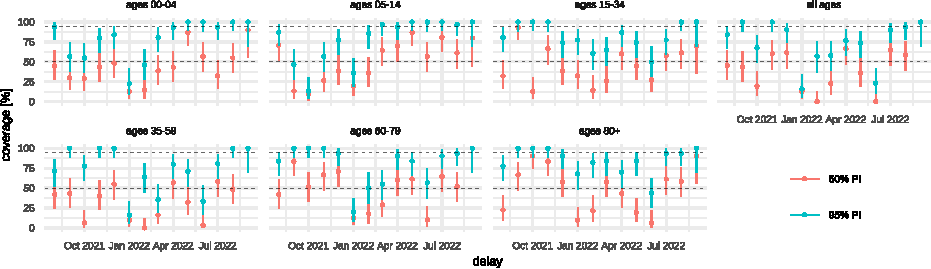
\includegraphics[width=\textwidth]{figures_tentative/coverages-1.pdf} 

}

\caption{Empirical coverage of 50\% and 95\% prediction intervals (PI) based on same-day nowcasts for dates 2021-08-01 to 2022-09-10 (406 dates) for which the true amount of hospitalisations after $12$ weeks is known as of the writing of this paper. We also display pointwise $95\%$ binomial confidence intervals for the coverage. Given the difficulties of real-time forecasting \cite{Desai2019Realtime} we deem the coverages good, except for the transitionary period in the end of 2021 where changing testing schemes and the change from Delta to Omicron cause our model to be overly confident. Coverage is generally better in the older age groups.}\label{fig:coverages}
\end{figure}

We further quantified uncertainties in estimaton by uncertainty
intervals based on an assumption of a (log)-normal distribution for the
errors with standard deviation based on past performance of our model.
In \cref{fig:coverages} we show the coverages of the \(50\%\) and
\(95\%\) prediction interval across all age groups and delays for the
whole time period of our study. For most age groups the \(50\%\)
prediction interval has close to nominal coverage, while the \(95\%\)
intervals have less than nominal coverage.

As our goal is to capture all of the uncertainty in this prediction, we
chose to assume a sensible distribution for the prediction, a normal
distribution for the two young age groups and a log-normal distribution
for all other age groups. This has the advantage of producing more
honest, wider, prediction intervals than those based on parametric
distributions. The estimated standard deviation will also account for
periods of low coverage, such as January 2022, albeit only after the
maximum delay of \(12\) weeks.

We base our choice of \(12\) weeks of delay on the empirical survival
function displayed in \cref{fig:delay_tails}. One could, however,
argue for shorter maximum delay such as \(6\) weeks because time from
reported infection to hospitalisation is much shorter, on the order of
\(\approx 10\) days \cite{Faes2020Time}, so hospitalisations after
this (shorter) period are unlikely to be due to the acute infection with
SARS-CoV-2. This would have two main benefits: The model would adapt
faster to changing circumstances and the indicator nowcasted describes
the severity of the epidemic more appropriately.

The main advantage of our model over established nowcasting approches is
its simplicity, making it easy to understand, straightforward to
implement and, once the reporting triangles for incidences and
hospitalisation are created, fast to run; taking only \(< XX\) minutes
on a standard notebook(\textbf{TODO: check!}).

The problem of nowcasting hospitalisations is different from previously
studied nowcasting settings in several ways. At the time of nowcast a
large fraction of hospitalisations are not only unobserved, but are yet
to occur - in this sense the nowcast is more accurately termed a
forecast. As the date of hospitalisation is not known, the
hospitalisations are associated by the date of reporting of the COVID-19
case, creating the double-weekday effect displayed in
\cref{fig:double_weekday_effect}. While daily updated data on
hospitalisations are available, these consist only of moving weekly
aggregates, consecutive observations are strongly auto-correlated.

We sidestep all of these issues by splitting the hospitalisations to
nowcast into weekly chunks, incorporating leading indicators of
hospitalisation -- the weekly reported case incidences -- and modelling
the number of hospitalisations to come in each chunk by binomial
thinning of incidences. Let us stress that this approach is only
possible in the special situation where case and hospitalisation are
explicitly linked, however we believe that incorporating leading
indicators into nowcasting models is a promising approach.

An additional advantage of our model is that the hospitalisation
probabilities can further be analysed, e.g.~by investigating association
between the publicly available vaccination rates and the probability of
hosptialisation and delay to hospitalisation. Sudden changes in these
fractions, as observed in 
\cref{fig:hospitalisation_probabilities_over_time}, can also hint towards
worse model performance, especially if this change can be attributed to
changing probability of hospitalisation due to new variants or changing
testing regime.

Real time forecasting of epidemiological indicators is a difficult task
\cite{Desai2019Realtime}, in particular quantifying uncertainty
\cite{Bracher2021Preregistered}. To test our model under real-time
circumstances we submitted daily nowcasts to the German COVID-19
NowcastHub \cite{2022Nowcasts} since Novemer 2021. In the nowcasting
context, \cite{Lawless1994Adjustments} goes to great lengths to
account for overdispersion due to changes in delay distribution,
introducing gamma and Dirichlet priors and explicitly modelling trends.
Such an approach would also be feasible for our approach, e.g.~model
incidences by an appropriate Poisson or negative binomial distribution
and, conditional on incidences, model hospitalisations by a binomial
distribution. As this increases the complexity of our model and relies
on the assumed distributions being sensible we opted for another
approach.

Regarding the indicator we stress that its value on a given date does
not represent the current occupancy of hospitals in Germany with
COVID-19 patients but is rather an approximation to the morbidity caused
by COVID-19 on that date. The reason for this discrepancy is that
hospitalisations are attributed to the reporting date of the associated
case, not that of hospitalisation. While the reporting date of the
hospitalisation can be recovered from the publicly available data, the
date of hospitalisation cannot. Additionally, no information on the
duration of stay is available, making it impossible to create an
indicator for the occupancy of hospitals based solely on data provided
by the \gls{rki}.

Implicit in all of these approaches is an assumption of
``stationarity'', i.e.~that future reported hospitalisations will behave
as they did in the past. Thus, all of these approaches might still be
insufficient if circumstances change drastically, for example
introduction of new testing schemes (school, 3G at workplace), changes
in the delay distribution due to new variants, or hospitals close to
capacity taking longer to process cases.

In summary, because models usually only capture a small part of the
highly dynamic data-generating process, we believe that uncertainty in
such circumstances should not come from unrealistic parametric
assumptions but rather be based on past model performance. Given the
discussed difficulties and the changing epidemiological dynamics in the
period studied, the observed errors of prediction (\cref{fig:REP})
and coverages of prediction intervals (\cref{fig:coverages}) are
satisfying.

In this paper we provide a straight-forward model for nowcasting
hospitalisations associated with COVID-19 in Germany. By leveraging
known incident cases, we can estimate fractions of hospitalisations in
weekly chunks which in turn avoids a complicated model of the two
weekday effects present in the data. As the circumstances of the
epidemic are changing constantly, e.g.~vaccination coverage, testing
regimes and emerging variants, we based uncertainty not on parametric
assumptions but on the past performance of our model, assuming a
(log)normal predictive distribution. We contributed nowcasts based on
this model since November 2021 to the German COVID-19 NowcastHub
\cite{2022Nowcasts}, a collaborative platform collecting and
aggregating such nowcasts from multiple research groups. The performance
of the nowcasts in this Hub and presented in this paper (\cref{fig:REP} and \cref{fig:coverages}) are, regarding the simplicity of
the model and the highly dynamic situation, quite satisfying.

There are multiple extensions to our model worth investigating. Firstly
hospitalisations are also available at the federal state level so
nowcasting on a spatial scale is naturally of interest due to
hetereogeneity in immunisation status and testing regimes across states.
However, splitting hospitalisations into six age groups and 16 federal
states will result in small numbers with larger variability which in
turn increases variabliity in estimates \(p_{t,d,k}\) and thus
predictions which may require some regularisation thus increasing the
models complexity. Secondly, in a similar vein, modeling the temporal
evolution of hospitalisation probabilities by smooth functions,
e.g.~splines
\cite{vandeKassteele2019Nowcasting,Schneble2021Nowcasting}, may help
in early detection of changing circumstances and thus lead to better
forecasts. Thirdly our uncertainty intervals account for the variance of
past performance, but \cref{fig:REP} suggests that there is
substantial bias in periods of changing circumstances which could be
incorporated into our model in a straightforward way. Finally to predict
the future course of the epidemic forecasting hospitalisations for dates
\(t\) that lie in the future is of interest, which could be accomplished
if one has a model that produces forecasts for incidences for all age
groups.